\chapter{优化问题初步}
    
\section{优化问题引入}

\begin{problem}
    \label{Problem:ClusteringCenter}
    假设$N$个样本向量$ x_{1}, \ldots, x_{N} \in \mathbb{R}^{n} $, 需要找到中心向量$z$满足

    $$ \min _{z \in \mathbf{R}^{n}} \sum_{i=1}^{N}\left\|x_{i}-z\right\|_{2}^{2} $$
\end{problem}

\begin{definition}[高阶无穷小记号 $o$]
    设 $ x, y $ 是同一变化过程中的无穷小, 即 $ x \rightarrow 0, y \rightarrow 0 $, 如果它们极限

$$
\lim_{x \rightarrow 0, y \rightarrow 0} \frac{y}{x}=0
$$

则称 $ y $ 是 $ x $ 的高阶无穷小, 记作 $ y=o(x) $.
\end{definition}

\begin{corollary}
    $$ \lim_{x \rightarrow 0, y \rightarrow 0} \frac{y}{C x}=\frac{1}{C} \lim_{x \rightarrow 0, y \rightarrow 0} \frac{y}{x}=0 $$

    也即则称 $ y $ 是 $ C x $ 的高阶无穷小, 记作 $ y=o(C x) $ . 
\end{corollary}

\begin{proposition}[优化求解的必要条件]
    假设函数$f$在$\hat{x}$可微, 则有

    $$ \hat{x}=\arg \min _{x \in \mathbb{R}^{n}} f(x) \Rightarrow \nabla f(\hat{x})=0 $$
\end{proposition}

\begin{proof}
    假设函数$f$在$\hat{x}$一阶泰勒展开, 有

    $$ f(x)=f(\hat{x})+\langle\nabla f(\hat{x}), x-\hat{x}\rangle+o\left(\|x-\hat{x}\|_{2}\right) $$

    假设$ \delta f(\hat{x}) \neq 0 $, 则令 $ \tilde{x}=\hat{x}-t \nabla f(\hat{x}), t>0 $,可得

    $$ f(\tilde{x})=f(\hat{x})-t\|\nabla f(\hat{x})\|_{2}^{2}+o\left(t\|\nabla f(\hat{x})\|_{2}\right) $$

    当 $ t \rightarrow 0 $ 则$ t\|\nabla f(\hat{x})\|_{2} \rightarrow 0 $,  高阶无穷小$ {o }^{\prime}\left(t\|\nabla f(\hat{x})\|_{2}\right) \rightarrow 0 $

    当$t$足够小时, 存在$ t\|\nabla f(\hat{x})\|_{2} \geq o\left(t\|\nabla f(\hat{x})\|_{2}\right) $, 即

    $$ -t\|\nabla f(\hat{x})\|_{2}^{2}+o\left(t\|\nabla f(\hat{x})\|_{2}\right) \leq 0 $$

    $$ f(\tilde{x})=f(\hat{x})-t\|\nabla f(\hat{x})\|_{2}^{2}+o\left(t\|\nabla f(\hat{x})\|_{2}\right) \leq f(\hat{x}) $$

    与 $ \hat{x}=\arg \min _{\mathbf{R}^{n}} f(x) $ 矛盾. 

    $ \nabla f(\widehat{x})=0 $, 是最优问题解的必要条件. 通常 $ \nabla f(\hat{x})=0 \not \Leftrightarrow \hat{x}=\arg \min _{\mathbf{R}^{n}} f(x) $. 
\end{proof}

\begin{example}
    $$ f(x)=-x^{2}, \quad x \in \mathbb{R}, \hat{x}=\operatorname{argmin}_{\mathbb{R}} f(x) $$

    $ \nabla f(\hat{x})=0 $, 则有 $ -2 \hat{x}=0 $, 即 $ \hat{x}=0 $

    $$ f(\hat{x})=0 \geq f(x), \quad x \in \mathbf{R} $$


\end{example}

\section{Convex Set}

\begin{definition}[凸集]
    $ \forall x, y \in \Omega, \alpha \in \mathbb{R}, 0 \leq \alpha \leq 1 $有

    $$ \alpha x+(1-\alpha) y \in \Omega $$

    则定义域$ \Omega \in \mathbb{R}^{n} $称为凸的(Convex)集合

    (域内两点连线之间都属于这个域)
\end{definition}

\begin{definition}[凸函数]
    设函数 $ f(x) $ 定义于称为\textit{凸的定义域} $ \Omega \in \mathbb{R}^{n} $满足

    $$ f(\alpha x+(1-\alpha) y) \leq \alpha f(x)+(1-\alpha) f(y), \forall x, y \in \Omega, \alpha \in \mathbf{R}, 0 \leq \alpha \leq 1 $$

    称其为凸函数. 
\end{definition}

% todo 图片

\begin{example}
    \label{Example:SquareIsConvex}
    $$ f(x)=x^{2}, x \in \mathbf{R} $$

    $$ \begin{aligned} f(\alpha x+(1-\alpha) y) &=(\alpha x+(1-\alpha) y)^{2} 
    \\ &=\alpha^{2} x^{2}+2 \alpha(1-\alpha) x y+(1-\alpha)^{2} y^{2} 
    \\ &=\alpha x^{2}+(1-\alpha) y^{2}+\left(\alpha^{2}-\alpha\right) x^{2}+\left(\alpha^{2}-\alpha\right) y^{2}+2 \alpha(1-\alpha) x y 
    \\ &=\alpha x^{2}+(1-\alpha) y^{2}-\alpha(1-\alpha)(x-y)^{2}
    \\ &\leq \alpha x^{2}+(1-\alpha) y^{2}=\alpha f(x)+(1-\alpha) f(y)
    \end{aligned} $$
\end{example}

\begin{example}
    \label{Example:NormIsConvex}
    $ f(x)=\|x\| $, 其中 $ \|  \cdot \| $ 表示 $ \mathbb{R}^{n} $ 上的向量范数, $ x \in \mathbb{R}^{n} $.
\end{example}

\begin{proof}
    \label{Example:L2NormIsConvex}
    $$ \|\alpha x+(1-\alpha) y\| \leq\|\alpha x\|+\|(1-\alpha) y\|=|\alpha|\|x\|+|1-\alpha|\|y\| $$
\end{proof}

\begin{example}
    $$ f(x)=\|x\|_{2}^{2}, x \in \mathbb{R}^{n} $$
\end{example}

\begin{theorem}[可微函数$f$是凸函数的充要条件]
    \label{Theorem:ConvexDiffential}
    $$ f(y) \geq f(x)+\langle\nabla f(x), y-x\rangle, \quad \forall x, y $$
\end{theorem}

\begin{proof}
    首先, 证明一维情况 $ f: \mathbb{R} \rightarrow \mathbb{R}, \alpha \in[0,1] $.

    $ \Rightarrow  $ 充分条件: $ f(\alpha x+(1-\alpha) y)=f(x+(1-\alpha)(y-x)) \leq \alpha f(x)+(1-\alpha) f(y) $,有

    $$ f(y) \geq f(x)+\frac{f(x+(1-\alpha)(y-x))-f(x)}{(1-\alpha)(y-x)}(y-x) $$

    令 $ \alpha \rightarrow 1^- $, 则有 $ f(y) \geq f(x)+f^{\prime}(x)(y-x) $.

    $ \Leftarrow  $ 必要条件:令 $ y \neq x, z=\alpha x+(1-\alpha) y$则有

    $$  f(x) \geq f(z)+f^{\prime}(z)(x-z), f(y) \geq f(z)+f^{\prime}(z)(y-z)  $$

    可得 
    $$\begin{aligned}
        \alpha f(x)+(1-\alpha) f(y) &\geq f(z)+\alpha f^{\prime}(z)(x-z)+(1-\alpha) f^{\prime}(z)(y-z) \\
        &=f(z)+f^{\prime}(z)(\alpha x+(1-\alpha) y-z) \\
        &=f(z)
    \end{aligned}
    $$

    证明 $ n $ 维情况 $ f: \mathbb{R}^{n} \rightarrow \mathbb{R} $.

    $ \Rightarrow $ 充分条件:令 $ g(t)=f(t x+(1-t) y), t \in \mathbb{R} $, 则 $ g^{\prime}(t)=\langle\nabla f(t x+(1-t) y), x-y\rangle $ 由于 $ f $ 是凸函数, 证明 $ g(t) $ 也是凸函数;并可得 $ g(0) \geq g(1)+g^{\prime}(1)(-1) $, 得证.

    $ \Leftarrow $ 必要条件:与一维类似. (将$f^{\prime}$改为$\nabla f(z)^T$) 
\end{proof}

\begin{theorem}
    如果可微函数$f$是凸函数, 则有

    $$ \hat{x}=\arg \min _{x \in \mathbb{R}^{n}} f(x) \Leftrightarrow \nabla f(\hat{x})=0 $$
\end{theorem}

\begin{proof}
    已证 $ \hat{x}=\arg \min _{x \in \mathbb{R}^{n}} f(x) \Rightarrow $ 可得 $ \nabla f(\hat{x})=0 $

    只需证 $ \nabla f(\hat{x})=0 \Rightarrow \hat{x}=\arg \min _{x \in \mathbb{R}^{n}} f(x) $.

    由于函数 $ f $ 是可微凸的, 则有 $ \forall x \in \mathbb{R}^{n} $,
$$
\begin{aligned}
f(x) & \geq f(\hat{x})+\langle\nabla f(\hat{x}), x-\hat{x}\rangle \\
& \geq f(\hat{x})+\langle 0, x-\hat{x}\rangle \geq f(\hat{x})
\end{aligned}
$$

可得 $ f(x) \geq f(\hat{x}), \hat{x}=\arg \min _{x \in \mathbb{R}^{n}} f(x) $.
\end{proof}

\section{向量偏导}

\begin{definition}[向量对向量的导数]
    \label{Definition:VectorVectorDerivative}
    $$ x=\left[\begin{array}{c}x_{1} \\ \vdots \\ x_{n}\end{array}\right], z=\left[\begin{array}{c}z_{1} \\ \vdots \\ z_{n}\end{array}\right] $$

    $$ \nabla f(z)=\left[\begin{array}{c}\frac{\partial f(z)}{\partial z_{1}} \\ \vdots \\ \frac{\partial f(z)}{\partial z_{n}}\end{array}\right] $$
\end{definition}

\begin{example}
    $$ f(z)=x^{T} z+z^{T} z=\sum_{i=1}^{n}\left\{x_{i} z_{i}+z_{i}^{2}\right\} $$

    它的导数是
    $$ \nabla f(z)=\left[\begin{array}{c}\frac{\partial f(z)}{\partial z_{1}} \\ \vdots \\ \frac{\partial f(z)}{\partial z_{n}}\end{array}\right]=\left[\begin{array}{c}x_{1}+2 z_{1} \\ \vdots \\ x_{n}+2 z_{n}\end{array}\right]=x+2 z $$
\end{example}


问题\ref{Problem:ClusteringCenter}中已知目标函数是凸函数. (见\ref{Example:SquareIsConvex}, \ref{Example:NormIsConvex}, \ref{Example:L2NormIsConvex})

则可以求解

\begin{proof}
    

$$ f(z)=\sum_{i=1}^{N}\left\|x_{i}-z\right\|_{2}^{2}=\sum_{i=1}^{N}\left\langle x_{i}-z, x_{i}-z\right\rangle=\sum_{i=1}^{N}\left\{x_{i}^{T} x_{i}-2 x_{i}^{T} z+z_{i}^{T} z\right\} $$

利用等价条件\ref{Theorem:ConvexDiffential}

$$ \nabla f(z)=\sum_{i=1}^{N}\left\{-2 x_{i}+2 z\right\}=0 $$ (求导 \ref{Definition:VectorVectorDerivative})

$$ z=\frac{1}{N} \sum_{i=1}^{N} x_{i} $$
\end{proof}
% todo (2021-11-02 19:29): another solution

另解:

\begin{proof}
    $ J\left(x_{0}\right)=\sum_{i=1}^{n}\left\|x_{0}-x_{i}\right\|^{2} , $ 其中 $ m=\frac{1}{n} \sum_{i=1}^{n} x_{i} $

    $$\begin{aligned}
        J\left(x_{0}\right)&=\sum_{i=1}^{n}\left\|\left(x_{0}-m\right)-\left(x_{i}-m\right)\right\|^{2} \\
        &=\sum_{i=1}^{n}\left\|x_{0}-m\right\|^{2}-2 \sum_{i=1}^{n}\left(x_{0}-m\right)^{T}\left(x_{i}-m\right)+\sum_{i=1}^{n}\left\|x_{i}-m\right\|^{2} \\
        &= \sum_{i=1}^{n}\left\|x_{0}-m\right\|^{2}-2\left(x_{0}-m\right)^{T} \sum_{i=1}^{n}\left(x_{i}-m\right)+\sum_{i=1}^{n}\left\|x_{i}-m\right\|^{2}
    \end{aligned}$$


因为
$$ \sum_{i=1}^{n}\left(x_{i}-m\right)=\sum_{i=1}^{n} x_{i}-n m=\sum_{i=1}^{n} x_{i}-n \cdot \frac{1}{n} \sum_{i=1}^{n} x_{i}=0 $$

所以有 $$ J\left(x_{0}\right)=\sum_{i=1}^{n}\left\|x_{0}-m\right\|^{2}+\sum_{i=1}^{n}\left\|x_{i}-m\right\|^{2} $$

即当$x_0$等于均值时,有最小均方.
\end{proof}

\section{标量优化问题:投影问题}

\begin{FigureCenter}{Projection onto a line}
   

\tikzset{every picture/.style={line width=0.75pt}} %set default line width to 0.75pt        

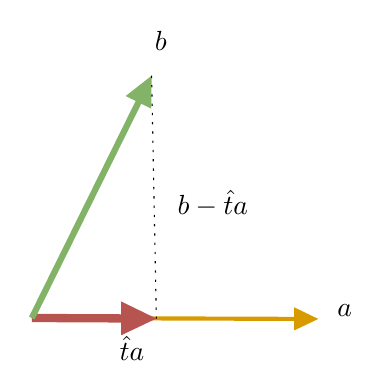
\begin{tikzpicture}[x=0.75pt,y=0.75pt,yscale=-1,xscale=1]
%uncomment if require: \path (0,300); %set diagram left start at 0, and has height of 300

%Straight Lines [id:da8764321810021003] 
\draw [color={rgb, 255:red, 215; green, 155; blue, 0 }  ,draw opacity=1 ][line width=1.5]    (152,230) -- (286,230.46) ;
\draw [shift={(290,230.47)}, rotate = 180.2] [fill={rgb, 255:red, 215; green, 155; blue, 0 }  ,fill opacity=1 ][line width=0.08]  [draw opacity=0] (11.61,-5.58) -- (0,0) -- (11.61,5.58) -- cycle    ;
%Straight Lines [id:da47866964225433306] 
\draw [color={rgb, 255:red, 184; green, 84; blue, 80 }  ,draw opacity=1 ][line width=3]    (152,230) -- (206,230.26) ;
\draw [shift={(212,230.29)}, rotate = 180.28] [fill={rgb, 255:red, 184; green, 84; blue, 80 }  ,fill opacity=1 ][line width=0.08]  [draw opacity=0] (16.97,-8.15) -- (0,0) -- (16.97,8.15) -- cycle    ;
%Straight Lines [id:da7728847142920288] 
\draw [color={rgb, 255:red, 130; green, 179; blue, 102 }  ,draw opacity=1 ][line width=2.25]    (152,230) -- (207.49,117.78) ;
\draw [shift={(209.71,113.29)}, rotate = 476.31] [fill={rgb, 255:red, 130; green, 179; blue, 102 }  ,fill opacity=1 ][line width=0.08]  [draw opacity=0] (14.29,-6.86) -- (0,0) -- (14.29,6.86) -- cycle    ;
%Straight Lines [id:da29849014601149504] 
\draw  [dash pattern={on 0.84pt off 2.51pt}]  (209.71,113.29) -- (212,230.29) ;

% Text Node
\draw (210,90.4) node [anchor=north west][inner sep=0.75pt]    {$b$};
% Text Node
\draw (193,237.4) node [anchor=north west][inner sep=0.75pt]    {$\hat{t} a$};
% Text Node
\draw (298,222.4) node [anchor=north west][inner sep=0.75pt]    {$a$};
% Text Node
\draw (221,167.4) node [anchor=north west][inner sep=0.75pt]    {$b-\hat{t} a$};


\end{tikzpicture}

\end{FigureCenter}


\begin{problem}
    假设$ a, b \in \mathbb{R}^{n}, a \neq 0, t \in \mathbb{R}$, 当$t$ 多大时, $ta$到$b$之间的距离最小

    $$ \hat{t}=\min _{t}\|t a-b\|_{2}^{2} $$
\end{problem}

    \begin{remark}
        t是标量,ta是向量.
    \end{remark}

    定义
    $$ f(t)=\|t a-b\|_{2}^{2}=\langle t a-b, t a-b\rangle=t^{2} a^{T} a-2 t a^{T} b+b^{T} b $$

    可以验证$f(t)$满足凸函数的定义。

    $$ \nabla f(t)=2 t a^{T} a-2 a^{T} b=0 $$

    $$ \hat{t}=\frac{a^{T} b}{a^{T} a}=\frac{a^{T} b}{\|a\|_{2}^{2}} $$





\begin{FigureCenter}{Projection onto a line from the prospective of linear algebra}
    \tikzset{every picture/.style={line width=0.75pt}} %set default line width to 0.75pt        

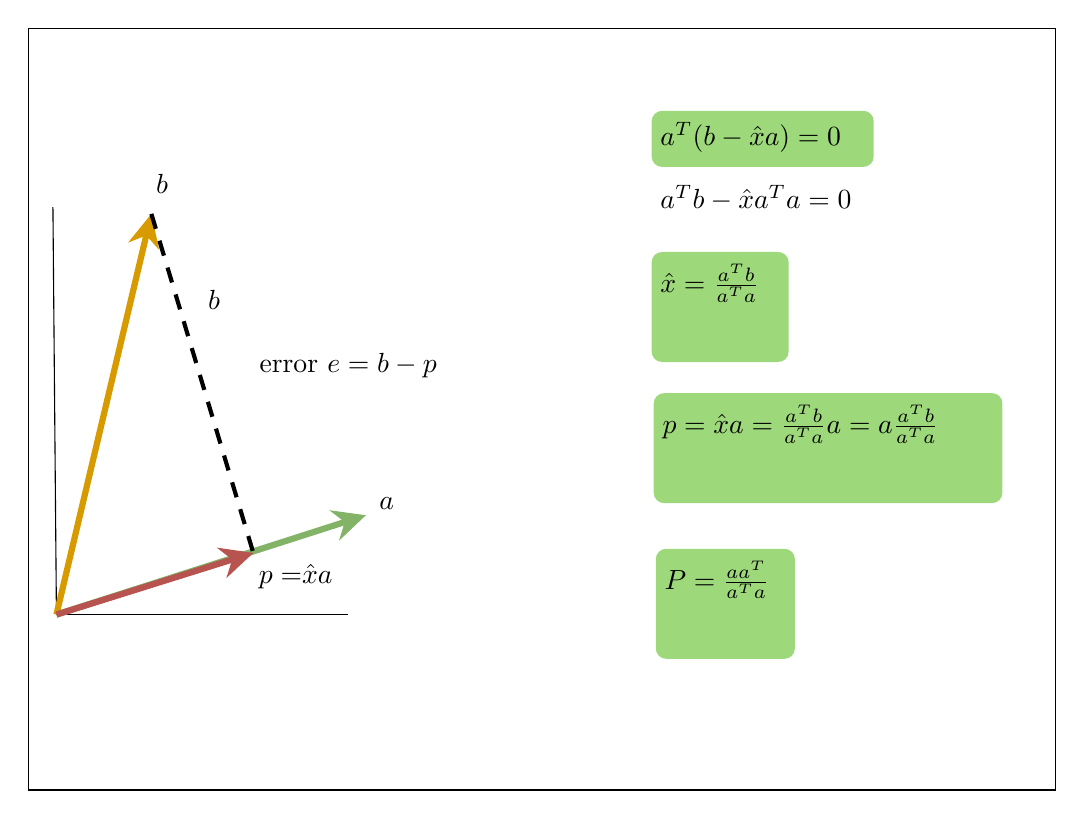
\begin{tikzpicture}[x=0.75pt,y=0.75pt,yscale=-1,xscale=1]
%uncomment if require: \path (0,371); %set diagram left start at 0, and has height of 371

%Straight Lines [id:da055809839407445105] 
\draw    (12.54,89.33) -- (14.23,285.69) ;
%Straight Lines [id:da12985171386013317] 
\draw    (14.23,285.69) -- (154.84,285.69) ;
%Straight Lines [id:da5377763269926785] 
\draw [color={rgb, 255:red, 215; green, 155; blue, 0 }  ,draw opacity=1 ][line width=2.25]    (14.23,285.69) -- (58.81,97.49) ;
\draw [shift={(59.97,92.63)}, rotate = 463.33] [fill={rgb, 255:red, 215; green, 155; blue, 0 }  ,fill opacity=1 ][line width=0.08]  [draw opacity=0] (16.07,-7.72) -- (0,0) -- (16.07,7.72) -- (10.67,0) -- cycle    ;
%Straight Lines [id:da49492424918304767] 
\draw [color={rgb, 255:red, 130; green, 179; blue, 102 }  ,draw opacity=1 ][line width=2.25]    (14.23,285.69) -- (158.55,239.37) ;
\draw [shift={(163.31,237.84)}, rotate = 522.2] [fill={rgb, 255:red, 130; green, 179; blue, 102 }  ,fill opacity=1 ][line width=0.08]  [draw opacity=0] (16.07,-7.72) -- (0,0) -- (16.07,7.72) -- (10.67,0) -- cycle    ;
%Straight Lines [id:da8103869094631817] 
\draw [color={rgb, 255:red, 184; green, 84; blue, 80 }  ,draw opacity=1 ][line width=2.25]    (14.23,285.69) -- (104.33,257.48) ;
\draw [shift={(109.1,255.99)}, rotate = 522.62] [fill={rgb, 255:red, 184; green, 84; blue, 80 }  ,fill opacity=1 ][line width=0.08]  [draw opacity=0] (16.07,-7.72) -- (0,0) -- (16.07,7.72) -- (10.67,0) -- cycle    ;
%Straight Lines [id:da03005700586607185] 
\draw [line width=1.5]  [dash pattern={on 5.63pt off 4.5pt}]  (59.97,92.63) -- (109.1,255.99) ;
%Shape: Rectangle [id:dp5894620344568704] 
\draw   (0.64,3.19) -- (495.64,3.19) -- (495.64,370.19) -- (0.64,370.19) -- cycle ;

% Text Node
\draw (61.02,72.24) node [anchor=north west][inner sep=0.75pt]    {$\boldsymbol{b}$};
% Text Node
\draw (110.52,260.07) node [anchor=north west][inner sep=0.75pt]    {$\boldsymbol{p=}\hat{x}\boldsymbol{a}$};
% Text Node
\draw (168.58,227.91) node [anchor=north west][inner sep=0.75pt]    {$\boldsymbol{a}$};
% Text Node
\draw (110.81,158.31) node [anchor=north west][inner sep=0.75pt]   [align=left] {error $\displaystyle \boldsymbol{e} =\boldsymbol{b-p}$};
% Text Node
\draw  [color={rgb, 255:red, 0; green, 0; blue, 0 }  ,draw opacity=0 ][fill={rgb, 255:red, 157; green, 217; blue, 123 }  ,fill opacity=1 ]  (301,48) .. controls (301,45.24) and (303.24,43) .. (306,43) -- (403,43) .. controls (405.76,43) and (408,45.24) .. (408,48) -- (408,65) .. controls (408,67.76) and (405.76,70) .. (403,70) -- (306,70) .. controls (303.24,70) and (301,67.76) .. (301,65) -- cycle  ;
\draw (304,47.4) node [anchor=north west][inner sep=0.75pt]    {$\boldsymbol{a^{T}( b} -\hat{x}\boldsymbol{a}) =0$};
% Text Node
\draw (304,77.4) node [anchor=north west][inner sep=0.75pt]    {$\boldsymbol{a^{T} b} -\hat{x}\boldsymbol{a^{T} a} =0$};
% Text Node
\draw  [color={rgb, 255:red, 0; green, 0; blue, 0 }  ,draw opacity=0 ][fill={rgb, 255:red, 157; green, 217; blue, 123 }  ,fill opacity=1 ]  (301,116) .. controls (301,113.24) and (303.24,111) .. (306,111) -- (362,111) .. controls (364.76,111) and (367,113.24) .. (367,116) -- (367,159) .. controls (367,161.76) and (364.76,164) .. (362,164) -- (306,164) .. controls (303.24,164) and (301,161.76) .. (301,159) -- cycle  ;
\draw (304,115.4) node [anchor=north west][inner sep=0.75pt]    {$\hat{x} =\boldsymbol{\frac{a^{T} b}{a^{T} a}}$};
% Text Node
\draw  [color={rgb, 255:red, 0; green, 0; blue, 0 }  ,draw opacity=0 ][fill={rgb, 255:red, 157; green, 217; blue, 123 }  ,fill opacity=1 ]  (302,184) .. controls (302,181.24) and (304.24,179) .. (307,179) -- (465,179) .. controls (467.76,179) and (470,181.24) .. (470,184) -- (470,227) .. controls (470,229.76) and (467.76,232) .. (465,232) -- (307,232) .. controls (304.24,232) and (302,229.76) .. (302,227) -- cycle  ;
\draw (305,183.4) node [anchor=north west][inner sep=0.75pt]    {$\boldsymbol{p} =\hat{x}\boldsymbol{a=\frac{a^{T} b}{a^{T} a} a=a\frac{a^{T} b}{a^{T} a}}$};
% Text Node
\draw (86.05,128.12) node [anchor=north west][inner sep=0.75pt]    {$\boldsymbol{b}$};
% Text Node
\draw  [color={rgb, 255:red, 0; green, 0; blue, 0 }  ,draw opacity=0 ][fill={rgb, 255:red, 157; green, 217; blue, 123 }  ,fill opacity=1 ]  (303,259) .. controls (303,256.24) and (305.24,254) .. (308,254) -- (365,254) .. controls (367.76,254) and (370,256.24) .. (370,259) -- (370,302) .. controls (370,304.76) and (367.76,307) .. (365,307) -- (308,307) .. controls (305.24,307) and (303,304.76) .. (303,302) -- cycle  ;
\draw (306,258.4) node [anchor=north west][inner sep=0.75pt]    {$\boldsymbol{P=\frac{\boldsymbol{a} a^{T}}{a^{T} a}}$};

\end{tikzpicture}
\end{FigureCenter}



\section{Clustering}

将物理或抽象对象的集合分成由类似特征组成的多个类的过程称为\textit{聚类(clustering)}.



目标:分成$k$个集合, 尽量使得同一个集合中的向量彼此接近. 

\begin{notation}
    给定N个n维向量 $ x_{1}, \ldots, x_{N} \in \mathbb{R}^{n} $

    \begin{itemize}
        \item 标签 $ c_{i} \in\{1,2, \cdots, k\} $ 表示向量 $ x_{i} $ 所属类别, 例如 $ c_{i}=2 $ 表示 $ x_{i} $ 属于第2类. 
        \item 对于 $ j=1, \ldots, k, \quad G_{j}=\left\{i: c_{i}=j\right\} $ 表示属于第j类的向量 $ x_{i} $ 的下标集合. 
        \item 向量 $ z_{j}, j=1, \ldots, k $, 表示同属于 $ j $ 类的向量 $ x_{i}, i \in G_{j} $ 的聚类中心. 
    \end{itemize}
\end{notation}

聚类目标是找到向量 $ x_{i} $ 的“标签 $ c_{i} $ ”和“聚类中心 $ z_{j} $ ”

\begin{problem}
    $$ \min _{z_{j}} \sum_{i \in G_{j}}\left\|x_{i}-z_{j}\right\|_{2}^{2}, j=1, \cdots, k $$

    $$ c_{i}=\underset{j=\{1, \cdots, k\}}{\operatorname{argmin}}\left\|x_{i}-z_{j}\right\|_{2}^{2}, i=1,2, \ldots, N $$

    
\end{problem}

$k$-means算法是将 $ \mathrm{N} $ 向量 $ x_{i} \in \mathbb{R}^{n} $ 划分成$k$类的迭代聚类算法. 

\begin{algorithm}
    \caption{$k$-means Algorithm}
    在 $ \mathrm{N} $ 个点中随机选取$k$个点, 分别作为聚类中心 $ z_{j} $\;
    更新聚类标签 $ c_{i} $ : 计算每个点 $ x_{i} $ 到k个聚类中心 $ z_{j} $ 的距离, 并将其分配到最近的聚类中心 $ z_{j} $ 所在的聚类中 $ c_{i}=j $\;
    更新聚类中心 $ z_{j} $ :重新计算每个聚类现在的质心, 并以其作作为新的聚类中心, 根据更新标签 $ c_{i} $, 更新属于第j类下标集合$ G_{j}=\left\{i: c_{i}=j\right\} $, 重新计算 $ c_{i} $ 类的聚类中心 $ z_{j} $\;
    重复步骤2、3, 直到所有聚类中心不再变化
\end{algorithm}

\begin{proof}
    更新聚类标签 $ c_{i} $:

    $$ \left\|x_{i}-z_{j}\right\|_{2}^{2}=\operatorname{argmin}\left\{\left\|x_{i}-z_{1}\right\|_{2}^{2},\left\|x_{i}-z_{2}\right\|_{2}^{2}, \cdots,\left\|x_{i}-z_{k}\right\|_{2}^{2}\right\} $$

    更新聚类中心 $ z_{j} $:

    $$ \nabla f_{j}\left(z_{j}\right)=\sum_{i \in G_{j}} 2\left(x_{i}-z_{j}\right)=0 $$
$$ z_{j}=\frac{1}{\left|G_{j}\right|} \sum_{i \in G_{j}} x_{i} $$

$ \left|G_{j}\right| $ 表示集合 $ G_{j} $ 中元素的数目. 
\end{proof}

在每一次迭代中目标函数$J$都会下降, 直到聚类中心 $ z_{1}, \cdots, z_{k} $ 和 划分聚类标签集合 $ G_{1}, \cdots, G_{k} $ 不再变化. 

但是k-means算法依赖于初始随机生成的聚类中心, 只可得到目标函数$J$的局部局部最优. 

解决方案:使用不同的(随机的)初始聚类中心运行k-means算法若干次, 取目标函数$J$值最小的一次作为最终的聚类结果. 

